% !Mode:: "TeX:UTF-8"

%%%%%%%%%%%%%%%%%%%%%%%%%%%%%%%%%%%%%%%%%%%%%%%%%%%%%%%%%%%%%%%%%%%%%%%%%%%%%%%%%%%%%%%


\documentclass{wreport}

%%%%%%%%%%%%%%%%%%%%%%%%基本信息填写%%%%%%%%%%%%%%%%%%%%%%%%%%%
\applicationyear{2024}  %%%%%%确定年份,用于页眉设置
%%%%%%%%%%%%%%%%%%%%%%%%%%%%%%%%%%%%%%%%%%%%%%%%%%%%%%%%%%%%


\begin{document}

%%%%%%%%%%%%%%%%%%%%%%%%%%%%%项目名称%%%%%%%%%%%%%%%%%%%%%%%%%%%%%
\section{项目名称}%不得更改
%%%%%%%%%%%%%%%%%%%%%%%%%%%%%%%%%%%%%%%%%%%%%%%%%%%%%%%%%%%%%%%%%
多智能体强化学习


%%%%%%%%%%%%%%研究工作的科学意义与拟解决的关键科学问题%%%%%%%%%%%%%%%%%%%
\section{研究工作的科学意义与拟解决的关键科学问题}%不得更改
%%%%%%%%%%%%%%%%%%%%%%%%%%%%%%%%%%%%%%%%%%%%%%%%%%%%%%%%%%%%%%%%

% !Mode:: "TeX:UTF-8"

\subsection{研究背景及意义}

21世纪以来,当前热点
\cite{cao2011formation}。


\subsection{文献说明}
多智能体系统协同编队控制作为多智能体系统协同控制技术的一个核心问题。
\subsubsection{说明}
% %%%%%%%%%%%%%%%%%正文%%%%%%%%%%%%%%%%%%%

\textcolor{red}{注意2:对于中文参考文献,为了保证格式正确,最好需在对应bib里面添加\text{language=\{zh\}},不加会默认当做英文文献处理。区别如图\ref{fig_bib0}。}

\begin{figure}[!htb]
  \centering
  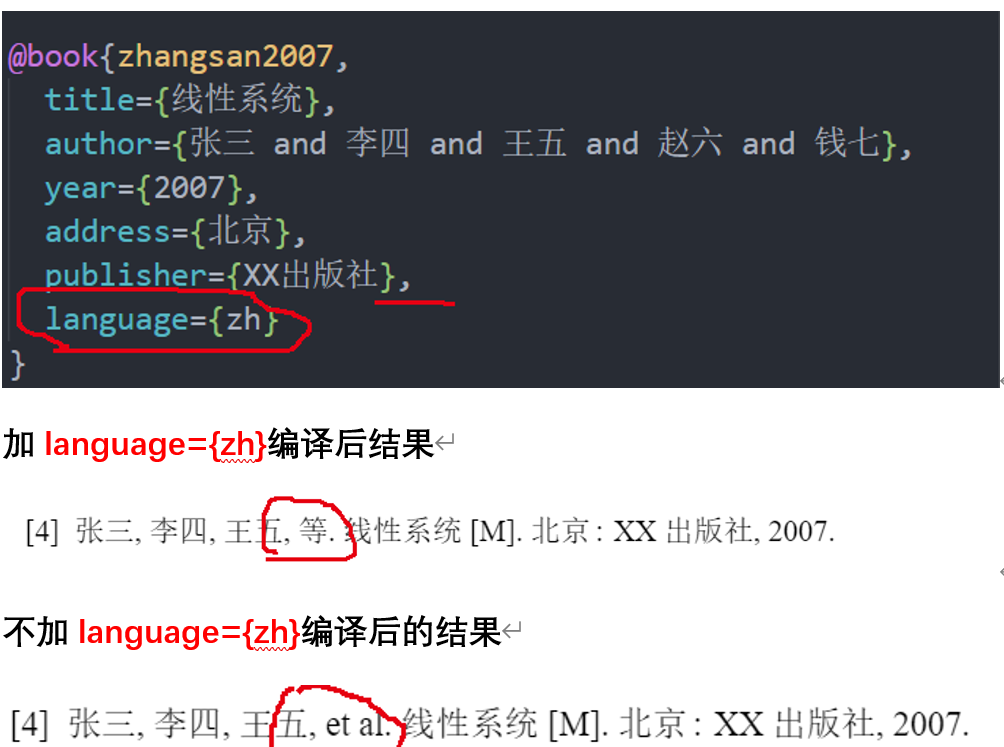
\includegraphics[width=1\textwidth]{中英文文献bib编译注意事项}
  \caption{中英文文献bib编译注意事项以作者超过3个为例进行说明}
  \label{fig_bib0}
\end{figure}

参考文献有两种格式引入\verb+\cite{}+以及\verb+\citep{}+。使用效果可见下面介绍:\\
1.插入会议inproceedings\cite{zhao2015bearing0}\\
2.插入教材课本book\cite{williams1991probability,chengzhaolin2006,zhangsan2007}\\
3.插入期刊article\cite{cao2011formation,xue2015formation}\\
4.插入硕博论文thesis\cite{lisi2015,wangwu2015,deans2005bearings}\\
5.插入网站misc\cite{irdawebsite,h7n9,wikipedia_moores_law}\\
6.插入专利patent\cite{xiao2012yi,p6915001}\\
7.插入新闻news报纸newspaper\cite{zhang2000,renminribao}\\
8.插入标准standard\cite{gbt3469-1983}

\textcolor{red}{注意1:参考文献格式不正确可能导致编译不通过,大家可以参考本工程中reference.bib中文献格式对网上下载不规范的bibtex文件进行修改。此外,如果上述类型里面条目有缺失会会导致编译不能输出正确格式。}



\subsection{插入表格}

\begin{table}[h]
    \caption{工作进度安排}
  \centering
  \setlength{\tabcolsep}{12mm}{
  \begin{tabular}{|c|c|c|}
  \hline
  序号 & 时间                  & 内容      \\ \hline
  1  & 20xx.1.8-20xx.1.12  & xxx     \\ \hline
  2  & 20xx.3.12-20xx.3.18 & xxx   \\ \hline
  \end{tabular}}
  \label{gra_process}
  \end{table}



%%%%%%%本项目研究目标,以及与申请者研究工作长期目标的关系%%%%%%%%%%%%%%
\section{本项目研究目标,以及与申请者研究工作长期目标的关系}%不得更改
%%%%%%%%%%%%%%%%%%%%%%%%%%%%%%%%%%%%%%%%%%%%%%%%%%%%%%%%%%%%%%%%
这部分写xxx




%%%%%%%%%%%%%%%%%%%项目研究内容,研究方案和进度安排%%%%%%%%%%%%%%%%%%%%
\section{项目研究内容,研究方案和进度安排}%不得更改
%%%%%%%%%%%%%%%%%%%%%%%%%%%%%%%%%%%%%%%%%%%%%%%%%%%%%%%%%%%%%%%%
这部分写xxx



%%%%%%%%%%%%%%%%%%%%%%%项目创新之处%%%%%%%%%%%%%%%%%%%%%%%%%%
\section{项目创新之处}%不得更改
%%%%%%%%%%%%%%%%%%%%%%%%%%%%%%%%%%%%%%%%%%%%%%%%%%%%%%%%%%%%%%%%
这部分写xxx



%%%%%%%%%%%%%%%%%%%%%%工作基础与工作条件%%%%%%%%%%%%%%%%%%%%%%%%%%
\section{工作基础与工作条件}%不得更改
%%%%%%%%%%%%%%%%%%%%%%%%%%%%%%%%%%%%%%%%%%%%%%%%%%%%%%%%%%%%%%%%
这部分写xxx



%%%%%%%%%%%%%%%%%%%%%预期研究结果%%%%%%%%%%%%%%%%%%%%%%%%%%%%%%%%
\section{预期研究结果}%不得更改
%%%%%%%%%%%%%%%%%%%%%%%%%%%%%%%%%%%%%%%%%%%%%%%%%%%%%%%%%%%%%%%%
这部分写xxx


%%%%%%%%%%%%%%%%%%%%%%%%%%%%%%%参考文献%%%%%%%%%%%%%%%%%%%%%%%%%% 
\myreference %不得更改
%%%%%%%%%%%%%%%%%%%%%%%%%%%%%%%%%%%%%%%%%%%%%%%%%%%%%%%%%%%%%%%%

\wbibliography{refs/reference}
%%%%%%%%%%%%%%%%%%%%%%%%%%%%%%%%%%%%%%%%%%%%%%%%%%%%%%%%%%%%%%%%



\end{document}